\title{AG 1 - Which objects can be constructed using a ruler and a compass?}
\author{hmys}
\date{14 07 2022}
\begin{document}
\maketitle

This is the first entry in what will be a sequence of posts explaining some of the most elementary concepts in algebraic geometry, as well as some relevant notions in (commutative) algebra. In this post we will develop some very elementary field-theory and use it to fully characterize which objects are constructible using a ruler and compass. This is very interesting. Questions like whether it is possible to create a square with the same area as a given circle, or which regular n-gons are possible to construct have been central since antiquity, so I think it is quite interesting that they can be answered using such simple methods. \newline

$\mathbb{Fields}$ are commutative rings where all elements have two-sided inverses. The prototypical example is Q, the rational numbers, where any element $\frac{p}{q}$ has the inverse $\frac{q}{p}$. Fields don't have any non-trivial ideals, and all morphisms between fields are consequently injective (kernels are ideals). Thus any morphism $f: K_{1} \to K_{2}$ can be seen as a way to identify the domain as a subfield of the target field. Prototypical examples are $Q \subseteq R \subseteq C$. \newline

The high-level overview of what we are going to do in this article is this: we're going to show that Q can be constructed using a ruler and compass. Then we are going to show that certain irrational numbe

\par
test $\lim_{0 \to 10} \frac{1}{2 + 0.001}$

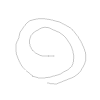
\includegraphics{drawing} 

\end{document}
